\documentclass[11pt]{article}

\usepackage{amsmath,amsthm,verbatim,amssymb,amsfonts,amscd, graphicx, amscd, mathrsfs}
\usepackage[english]{babel}
\usepackage[utf8x]{inputenc}
\usepackage[T1]{fontenc}
\usepackage{color}
\usepackage{listings}
\usepackage{lmodern}
\usepackage[colorlinks=true, allcolors=blue]{hyperref}
\usepackage{caption}
\usepackage{geometry}
\usepackage{graphicx}
\usepackage{multicol}
\usepackage{float}
\usepackage[round]{natbib}

\graphicspath{ {img/} }

\geometry{
  paper=a4paper, % Change to letterpaper for US letter
  top=1.5cm, % Top margin
  bottom=1.5cm, % Bottom margin
  left=2cm, % Left margin
  right=2cm, % Right margin
  %showframe, % Uncomment to show how the type block is set on the page
}

\renewcommand{\bf}[1]{\textbf{#1}}
\renewcommand{\it}[1]{\textit{#1}}
\renewcommand{\tt}[1]{\texttt{#1}}
\renewcommand{\rm}[1]{\mathrm{#1}}
\renewcommand{\sp}[1]{\textsuperscript{#1}}
\renewcommand{\p}{^{\prime}}
\renewcommand{\Fobs}{F^{\rm{obs}}}
\renewcommand{\tobs}{t_{\rm{obs}}}
\renewcommand{\thetaobs}{\theta_{\rm{obs}}}
\renewcommand{\Ms}{M_{\odot}}
\renewcommand{\fig}[4]{
\begin{figure}[H]
\begin{center}
\includegraphics[width=#2\linewidth]{#1}
\caption[#4]{#3}
\label{#1}
\end{center}
\end{figure}
}

\renewcommand{\eq}[2]{
\begin{equation}
\label{#1}
#2
\end{equation}
}

\renewcommand{\cen}[1]{
  \begin{equation}
  #1
  \end{equation}
}

\renewcommand{\xx}[1]{{x_{#1}}}

\renewcommand{\glo}[3]{
\bf{#1 (\it{#2}). }#3
}

\renewcommand{\bar}[1]{{\overline{#1}}}
\def \bangle{ \atopwithdelims \langle \rangle}

\lstset{ %
  backgroundcolor=\color{white},   % choose the background color; you must add \usepackage{color} or \usepackage{xcolor}
  basicstyle=\small,        % the size of the fonts that are used for the code
  commentstyle=\color{blue},    % comment style
  extendedchars=true,              % lets you use non-ASCII characters; for 8-bits encodings only, does not work with UTF-8
  keepspaces=true,                 % keeps spaces in text, useful for keeping indentation of code (possibly needs columns=flexible)
  keywordstyle=\color{red},       % keyword style
  language=Fortran,                 % the language of the code
  rulecolor=\color{black},         % if not set, the frame-color may be changed on line-breaks within not-black text (e.g. comments (green here))
  showspaces=false,                % show spaces everywhere adding particular underscores; it overrides 'showstringspaces'
  showstringspaces=false,          % underline spaces within strings only
  showtabs=false,                  % show tabs within strings adding particular underscores
  stringstyle=\color{green},     % string literal style
  tabsize=2,	                   % sets default tabsize to 2 spaces
  frame=single
}

%%%%%%%%%%%%%%%%%%%%%%%%%%%%%%%%%%%%%%%%%%%%%%%%%%%%%%%%%%%%%%%%%%%%%%%%%
%%%%%%%%%%%%%%%%%%%%%%%%%%%%%%%%%%%%%%%%%%%%%%%%%%%%%%%%%%%%%%%%%%%%%%%%%
%%%%%%%%%%%%%%%%%%%%%%%%%%%%%%%%%%%%%%%%%%%%%%%%%%%%%%%%%%%%%%%%%%%%%%%%%
\begin{document}

\bibliographystyle{plainnat}

\begin{center}

{\huge The Afterglow of the August 17\sp{th} 2017 Binary Neutron Star Merger Multi-messenger Event}

Raphaël Duque

\end{center}

\newpage

\section*{Summary}


\vfill

\section*{Résumé}

\newpage

\section*{Acknowledgments}


\tableofcontents

\newpage

\quad

\newpage
\pagenumbering{arabic}
\part{Introduction}

\section{MMT170817 -- a historical event}
On August 17\sp{th} 2017, the first binary neutron star merger event was observed through gravitational waves and electromagnetic signals. These observations pertain to a new paradigm of astronomy, namely \it{multi-messenger astronomy}. Hence, we will refer to the collection of these observations as MMT170817, for \it{Multi-Messenger Transient 170817}.

MMT170817 is the outcome of an extraordinary instrumental effort provided by each of the fields of this multi-messenger astronomy. The detection of gravitational waves has ground-breakingly entered the astronomical landscape in September of 2015, as gravitational waves from all three phases (inspiral, merger, ring-down) of the coalescence of a binary black hole were detected in the \it{two} interferometers of the LIGO Scientific Collaboration. After a total of five such two-instrument detections, the gravitational interferometer network was augmented with the French-Italian Virgo instrument on August 1\sp{st} 2017.

On August 17\sp{th}, a gravitational wave detection by this \it{three}-instrument configuration occurred. This signal is associated with the inspiral phase of the merger of a binary neutron star. This joint detection allowed for the first-in-history astronomically significant gravitational wave triangulation of the source in the sky. This triangulation is given in terms both of sky-projected position and distance, drawing a three dimensional error box in the Universe.

With a slight delay with respect to the gravitational wave determined time of merger, the Fermi Gamma-ray Space Telescope and the INTEGRAL space observatory detected a weak short gamma ray burst, itself triangulated to a sky-position consistent with that indicated by the gravitational waves.

A prompt but meticulous optical search for a new electromagnetic source in the gravitational wave 3D error box led to the first ever direct observation of a kilonova --~neutron-rich matter ejected from the system and which is the site of heavy element nucleosynthesis~--, and of a strongly atypically-behaved multi-wavelength afterglow, the observation of which carries on at the time of writing. The observations of these electromagnetic counterparts and the identification of NGC4993 as the host galaxy of the event were done by a hitherto unseen joint effort from the astronomical community as a whole, mobilizing an impressive amount of ground- and space-based instrumental resources. The cover page illustrations show the detection images of these electromagnetic counterparts in the infra-red, X-ray and radio bands.

The gravitational waves, gamma ray burst and other counterparts of this event are unambiguously associated, and thus are the multi-messenger manifestation of the first binary neutron star merger witnessed directly.

\section{Description of the multi-messenger observations of MMT170817}

\subsection{GW170817: gravitational waves from the inspiral phase}

The inspiral phase gravitational waves (GW) were detected for the $\sim$~3000 last orbits of the binary\footnote{The information contained in this subsection was synthesized from the GW detection publication \citep{23}.}. This signal GW170817, reproduced Figure \ref{gw}, lasted $\sim$~100~s and ended at 12:41:04.4~UTC. It is the loudest gravitational wave signal detected yet, with a signal-to-noise ratio of 32.4. The GW signal infers masses in the ranges of 0.86~--~1.36 $\Ms$ and 1.36~--~2.26 $\Ms$ for the two initial components (at 2$\sigma$). Given the ranges of measured galactic black hole masses, which are substantially higher than these, and the measured masses of some galactic binary neutron stars, which are consistent with these, a binary neutron star is the most likely nature of the GW progenitor. This is further supported by the detection of electromagnetic counterparts to this GW signal, indicating the presence of matter in the circum-merger environment after the merger, and thus the unlikeliness of a binary black hole progenitor. In fact, the uncertainty as to the exact nature (neutron star binary or black hole-neutron star binary) stems from the uncertainty on the maximum mass for a neutron star --~roughly between 2 to 3 solar masses~--, which is determined by the still uncertain equation of state (EOS) of neutron star material. In the signal of GW170817, the tidal deformabilities of both the components of the initial binary have been measured in the last orbits to be marginally consistent with a black hole-neutron star progenitor, but more largely consistent with those predicted by typical neutron star EOSs. This once again points to a binary neutron star progenitor for GW170817.

The Virgo detector did not measure a significant signal. This greatly constrained the localization of the source in the sky to a projected error box of 29~deg\sp{2}, and likely greatly decreased the duration of subsequent searches for electromagnetic counterparts.

The GW-inferred luminosity distance to the source is $40_{-14}^{+8}$~Mpc, making of the GW and short gamma ray burst the closest such events ever detected. This distance is further refined by combining GW data with EM observations of the host galaxy to $42.9\pm3.2$~Mpc. Similarly, the combination of the GW and EM data provides a viewing angle $\thetaobs$ (from our light-of-sight to the angular momentum of the binary) constrained to being less than 28~deg.

An essential feature of GW170817 is the non-detection of a postmerger ring-down signal, i.e the gravitational radiation emitted by the remaining central compact object during its relaxation to its state of equilibrium. This non-detection signifies either that the corresponding radiation was not emitted or intrinsically weak, which would likely be the case if the remaining object is a neutron star, or that the interferometer signal was to weak to be picked up. Moreover, had the final object been a black hole, its ring-down signal would have peaked at frequencies well out of the detectors' sensitive bands, given the masses at hand. In any event, the nature of the final object is undetermined by the GW signal.

\fig{gw}{1.0}{Spectrogram of a combination of both LIGO interferometers' data from GW170817 \citep{37}. Note the non-detection of a ring-down signal. The peak luminosity of the GW event is $\sim~9~\Ms c^2$/s \citep{49}.}{Spectrogram of a combination of both LIGO interferometers' data from GW170817}


\subsection{AT 2017gfo: the kilonova}
\label{kilonova}
The optical counterpart designated by the International Astronomical Union as AT 2017gfo (i.e the 4950\sp{th} astronomical transient of the year 2017) was discovered $\sim$~11~h after the merger event\footnote{The information contained in this subsection was synthesized from the multi-messenger detection publication \citep{51}.}. It was located in the lenticular galaxy NGC4993 within the ESO~508 group of galaxies in Hydra. Upon discovery, the $r$ band magnitude was measured to $\sim$~17, equivalent to an absolute magnitude of --16.

In the following days, until dimming to non-detection limits of AT 2017gfo, spectra of the transient were measured. The time evolution of these spectra is illustrated Figure \ref{kn}. These are associated with thermal radiation of an optically thick mass of dynamical (or tidal) ejecta from the merger event. It is understood that the neutron-rich matter ejected by the merger event is the site of $r$-process nucleosynthesis, that is the synthesis of neutron-rich heavy nuclei by rapid neutron capture in a neutron-dense environment, and the subsequent decay of these nuclei to heavy elements such as the lanthanides and actinides. The decay of the nuclei are a heat source within the kilonova, and the extremely opaque medium composed of heavy nuclei ensures its thermalization. What's more, the sudden decompression of this once-neutron-star material into the rarefied external medium drives the rapid expansion of the ejecta.

This vision is further supported by the claim to the detection of atomic cesium and tellurium ($Z = 55$ and $52$) absorption lines in the transient's spectrum \citep{53}.

\begin{figure}
    \centering
    \begin{subfigure}
        \centering
        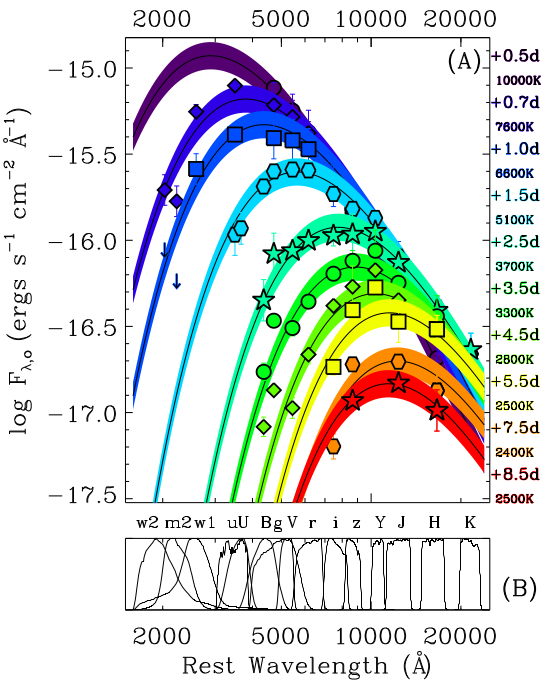
\includegraphics[width=0.48\linewidth]{kn}
    \end{subfigure}
    \begin{subfigure}
        \centering
        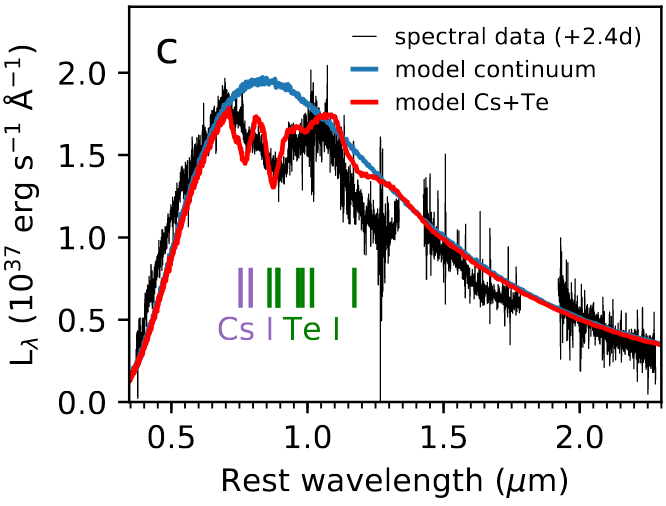
\includegraphics[width=0.48\linewidth]{cste}
    \end{subfigure}
    \caption[Spectra of AT 2017gfo]{\it{Left:} Time evolution of the spectrum of AT 2017gfo \citep{38}. \it{Right:} VLT/Xshooter visible and near-IR spectrum of the kilonova 2.4 days post-merger, where TeI and CsI absorption lines are claimed to have been found \citep{53}.}
    \label{kn}
\end{figure}

Some authors have argued in favor for two thermal components in the continuum spectrum of the kilonova \citep{57}. According to this vision, the redder component is more opaque due to the higher concentration of lanthanides ($Z = 57 \text{ to } 71$) with respect to the bluer component. Also, the redder component would originate in the dynamical ejection of matter upon merger, whereas the blue component would occur within a neutrino-driven wind lifted above an accretion disk around the final central object.


\subsection{GRB170817A: the gamma-ray burst}
The gamma ray burst (GRB) event started 1.72~s after the GW data merger time\footnote{The information contained in this subsection and the next was synthesized from the GRB detection publication \citep{52}.}. The distribution of GRBs according to their duration reveals a \it{bimodal distribution}. The \it{long} GRBs, with durations more than 2.0~s, which are consistently found hosted in star-forming galaxies, and the \it{short} GRBs, which show no correlation with the morphology of their host galaxies \citep[see][for a review]{28}. This has led the GRB community to suspect binary neutron star mergers as progenitors for short GRBs, as these merger events occur in galaxies with delays on the order of hundreds of million years --~the typical inspiral time for a binary~-- with respect to star forming episodes. The case of GRB170817A coincident with a GW signal from a binary inspiral goes to confirm this vision.

The duration of GRB170817A was 2.0~s, placing it in the class of short GRBs with a confidence level of $\sim$~72\%. GRB170817A's total isotropic-equivalent radiated energy was $\sim$~$10^{47}$~erg, around 4 orders of magnitude weaker that typical short gamma ray bursts, though photons with energies as high as 185~keV were emitted.

Moreover, it appears that the light curve of GRB170817A presents two successive components, one lasting 0.58~s, and a later second lasting 1.1~s. Spectrally, the first component resembles a typical non-thermal short GRB emission, and the second on the other hand is best fit by a thermal emission of temperature $\sim$~10\sp{7}~K (1 keV), though the significance of this spectral fit is debated and other spectral models are not excluded.

Furthermore, as illustrated in Figure \ref{yonetoku}, GRB170817A is an outlier of the $E_p$-$L_{\rm{iso}}$ relation, also know as the Yonetoku relation \citep{35}. In this relation which is broadly respected by short GRBs, $E_p$ is the peak of the spectrum of the GRB emission at the moment of its peak --~also considered as the energy of the photons which carry the bulk of the energy of the GRB~--, and $L_{\rm{iso}}$ is the isotropic equivalent luminosity of the burst at this moment. According to the Yonetoku relation, they are positively correlated.

Given an observed $(E_p, L_{\rm{iso}})$ couple, one may determine the values of these parameters which would have been measured if the event had been viewed under a different angle, using the general viewing-angle-dependent form of the Doppler factor $\mathcal{D}(\Gamma, \theta)$ (see Eq.~\ref{doppler} for details). Even when correcting for the possibly non-zero viewing angle, and placing the burst as seen closer to its axis --~as is done in Figure \ref{yonetoku}~--, GRB170817A remains an outlier of the Yonetoku relation.

\fig{yonetoku}{0.7}{The Yonetoku relation for the Swift BAT 4 catalog bursts \citep[black crosses: short GRB sample by][yellow line and band: best-fit correlation for a large sample of short and long GRBs, \it{ibid.}]{36} and GRB170817A \citep[red crosses][]{52}. The values of $E_p$ and $L_{\rm{iso}}$ that would have likely been measured for other viewing angles and an indicative Lorentz factor of 100 are indicated by red dots. The case of the GW-inferred maximum viewing angle $\thetaobs^{GW} = 28$~deg is indicated for reference.}{The Yonetoku relation for the Swift BAT 4 catalog bursts and GRB170817A}

These remarks indicate the \it{atypical} character of GRB170817A. More precisely, they lead to interrogations on the emission processes responsible for GRB170817A. Standard understandings of GRBs (the bulk of which occur at cosmological distances) imply relativistic jets seen along their axis and energy dissipation into gamma radiation therein. Is GRB170817A comprehensible in such standard models? Is it a particular case of these models? Can its weakness be explained by our seeing it off-axis? Or does it --~and possibly other GRBs from binary mergers~-- require a specific modeling? In our work, we will not be concerned with these questions, as we will focus on the afterglow of MMT170817. Nonetheless, these are central questions for the future study of neutron star mergers and their link to the population of GRBs.

A few other intrinsically weak GRBs have been observed in the past. An example is GRB980425 which stood out as an atypical event among long GRBs for its low luminosity. It was then found by \citet{50} that the internal shock model allowed such events, provided the outflow be slower and less energetic.


\subsection{The afterglow signal}
\label{ags}
Counterparts in the X-ray and radio bands were detected to significant levels 9 days and 15 days post-merger. When the kilonova signal had sufficiently decayed at 150 days post-merger, an optical band afterglow was also detected as emerging from the dimming kilonova signal.

The afterglow photometry points in these bands until $\sim$~250~d post-merger are reported Figure \ref{ag}. Among these photometry points, the latest ones --~and in particular those of the peak of the flux~-- were measured in the course of the work presented in this document. An essential feature of these afterglow light curves are their homothetic structure, i.e their seems to exist a time-independent index $k$ such that for two frequencies $\nu$ and $\nu\p$, we have $F_\nu = \left( \frac{\nu}{\nu\p} \right)^k F_{\nu\p}$. From these light curves, we can already infer $k \sim -0.5$.

\fig{ag}{0.5}{Afterglow photometry points in various bands \citep{29}. Notice the homothetical structure of the flux from band to band. In the optical band, the afterglow signal only appears after the dimming of the kilonova, and approximately coincides with the beginning of this work.}{Afterglow photometry points in various bands}

As we will shortly see, this structure is a first indication of which radiation process is at play in the afterglow --~synchrotron radiation~--, and allows us to consider for our study the light curve of only one band.


Another important feature of this afterglow emission is that it is long-lived. Indeed, the radio flux increased steadily until $\sim$~160~days post-merger, then commenced a steady decrease and is still observed at the time of writing. A comparison of the afterglow of MMT170817 with some short GRB afterglows from the total Swift catalog can be done using Figure \ref{remnants}. It is evident that MMT170817 is peculiar with respect of all of these.

\fig{remnants}{0.8}{Some short GRB afterglows from the Swift catalog \citep[blue lines, Swift X-ray Telescope data][]{61}. A quick comparison with the afterglow of MMT170817 on Figure \ref{ag} shows that this afterglow is like no other.}{Some short GRB afterglows from the Swift catalog}

\section{Goal of this work: an insight on the geometry and dynamical structure of the remnant of MMT170817 through its afterglow}

The merger of a binary neutron star is a complex phenomenon. It implies various physical components (compact objects, jets, ejectas, winds) which are subject to many dynamical and radiative processes (shock formation, nuclear processes, synchrotron emission, etc.). A coherent description of the binary neutron star merger phenomenon, from the inspiral phase to the electromagnetic afterglow, is still to be found. Most likely, the combination of all the multi-messenger observations from a large number of binary merger events probing their exterior diversity (viewing angle, external density) will be necessary to obtain this accurate description. In addition, each signal from a multi-messenger batch of observations bares the signature of the state of the system at different times.

During the merger event, matter is ejected from the system. It can be ejected by the collision of the neutron stars, by tidal forces before the merger, by the relaxation activity of the remaining central object after the merger, etc. This matter may assume various geometries --~spherical, jet-like~--, and be ejected with different dynamical structures --~all at once with a single velocity, with a distribution of velocities, in many ejection phases, etc. This matter, if ejected with speeds larger than that of sound, will form a shock in the circum-merger medium, producing an afterglow emission to the merger event, driven by an energized population of electrons at the shock front.

Thus, the afterglow emission holds information on the state of the system at late times, and is a first step one may take to approach the event in its entirety. This work is a spark for the study of the merger of binary neutron stars. Focusing on the afterglow, we will through modelization attempt to a first understanding of this event. In particular, we will search a coherent description of the outflow of matter responsible for the afterglow --~its geometry and dynamical structure~-- and give some first answers to the question of whether a relativistic jet was produced during the event.\\

The questions this work addresses are thus the following:

\begin{enumerate}
	\item \it{What is the geometry and the structure of the outflow of matter responsible for the afterglow?}
	\item \it{What are the characteristics of the circum-merger medium which this outflow penetrates?}
	\item \it{By which means is the kinetic energy dissipated into the afterglow radiation?}
	\item \it{Was a relativistic jet produced in the merger event?} This is a fundamental question the answer to which is a first step in linking the population of short GRBs with the phenomenon of binary neutron star mergers.
	\item \it{Which afterglow signals would we have seen, had we seen the event from a different viewing angle?}
\end{enumerate}


\part{Modelling the afterglow of MMT170817}

%\begin{multicols}{2}
\bf{Note on the physical origin of the afterglow.} As insisted upon in the introduction, MMT170817 is an \it{atypical} event. Nonetheless, the numerous observations of remnants and afterglows of transient electromagnetic events (such as supernovae and gamma ray bursts) indicate a common explanation of afterglows having timescales from days to years, such as that of MMT170817. Matter which is ejected during the previous phases of the phenomenon travels in the local external medium faster than the speed of sound. A shock thus forms at the interface of this shock with the interstellar medium. Interstellar material accumulates at this shock front, is excited and radiates. As the material accumulates, the shock decelerates. The exact nature and origin of the ejected matter, and the characteristics of the medium in which it evolves depends on the specific astrophysical phenomena at hand.

Thus, the models which we will describe here and later confront to observations will concern the radiation of interstellar material which is shocked and radiates through the synchrotron process at the front of a shock formed by the piston effect of ejecta from the merger on the exterior medium, while this shock decelerates as it penetrates the ISM.

\fig{shock}{0.5}{Cut across the shock front, showing the ejected matter, and the interstellar material accumulating a the shock front.}
\section{The physics of afterglows: deceleration dynamics, radiation and astronomical observables}

In this section, we will review the physics which will take part in the modelling of the afterglow of MMT170817. We will successively describe the deceleration of the remnant expanding in the interstellar medium, the radiation of matter at the shock front, and derive the electromagnetic signals which arise from this radiation. The more technical details of these physical processes may be found in \it{Appendix B}.

\subsection{Relativistic deceleration}

We now describe the dynamics of the deceleration of the remnant in the ISM. We will consider for this work two different structures for the ejected matter: a \it{mono-kinetic ejecta}, or a \it{radially stratified ejection}.

We will follow the Lorentz factor $\Gamma(r)$ of the ejected matter once it has reached the exterior radial coordinate $r$.

\bf{Mono-kinetic ejection.} In this case, the matter is ejected with initial energy $E_0$ and a single Lorentz factor $\Gamma_0$. By plowing through the ISM, the shock sweeps up interstellar material and decelerates. By denoting $M_{\rm{ej}}$ the mass of the ejected matter, $m(r)$ the accumulated mass swept up by the shock at radius $r$ from the point of ejection, conservation of energy implies that the initial total energy $\Gamma_0 M_{\rm{ej}} c^2 + m(r) c^2$ is distributed in the ejected mass energy $\Gamma(r) M_{\rm{ej}} c^2$ and the internal energy of the swept up mass $\Gamma(r)^2 m(r) c^2$. Thus:

$$\Gamma(r)^2 m(r) + \Gamma(r) M_{\rm{ej}} = \Gamma_0 M_{\rm{ej}} + m(r) $$

Details on the $\Gamma^2 m c ^2$ form for the thermal energy of the swept-up mass can be found in \it{Appendix B}.


We will consider for our purposes a homogeneous medium with numeric density $n$.

Suppose that the mass $M_{\rm{ej}}$ was ejected into a solid angle $\Omega$ by the central source, for instance in the form of a cone. Then if we neglect any lateral expansion of the ejected matter, the swept us mass at radius will be\footnote{In all generality, we should consider the average mass per particle in the local exterior environment instead of $m_P$.}:

$$m(r)~=~\Omega\int_0^r dr' r' ^ 2 n m_P$$

Thus by introducing the isotropic-equivalent ejected mass $M_{\rm{iso}} = 4\pi M_{\rm{ej}}/ \Omega$, the dimensionless mass parameter $\mu(r) \equiv \frac{m(r)}{M_{\rm{iso}}/\Gamma_0}$, writes:

\[
\begin{array}{lcr}

\mu(r) &= &\frac{\Omega\int_0^r dr' r' ^ 2 n m_P}{M_{\rm{ej}}/\Gamma_0}  \\
 &=& \frac{4\pi r ^ 3}{3 M_{\rm{iso}}/\Gamma_0} n m_P

\end{array}
\]

which no longer depends on the solid angle of ejection.


We may identify the \it{deceleration radius}, $R_{\rm{dec}} = \left( \frac{3 E_0}{4\pi n m_P \Gamma_0^2 c^2}\right) ^ {1/3}$, such that:

$$\mu(r) = \left( \frac{r}{R_{\rm{dec}}} \right)^3 $$

And finally, the solution for $\Gamma(r)$ is easily found to be:

$$\Gamma(r) = \Gamma_0 \frac{-1 + \sqrt{1 + 4\mu(r) + \frac{4\mu(r) ^ 2}{\Gamma_0^2}}}{2 \mu(r)}$$

\bf{Phases of deceleration.}We observe three phases in the deceleration of the shock front:

\begin{enumerate}
	\item For $\mu(r) \ll 1/4$, i.e. $r \ll R_{\rm{dec}}$, in the \it{coasting phase}, no deceleration occurs:

	\cen{$\Gamma(r) \simeq \Gamma_0$}

	\item For $1/4 \ll \mu(r) \ll \Gamma_0 ^ 2$, i.e. $R_{\rm{dec}} \ll r \ll \Gamma_0^{2/3} R_{\rm{dec}} \equiv R_{\rm{N}}$ (\it{newtonian radius}), the front is in a \it{relativistic deceleration phase}, during which the swept-up mass progressively reaches $\Gamma_0 M$:

	\cen{$\Gamma(r) \simeq \frac{\Gamma_0}{\sqrt{\mu(r)}} = \Gamma_0 \left(\frac{r}{R_{\rm{dec}}} \right) ^ {-3/2}$}


	\item For $\Gamma_0^2 \ll \mu(r)$, i.e. $ R_{\rm{N}} \ll r$:

	\cen{$\Gamma(r) \simeq 1$}

	and

	\cen{$\beta(r) \simeq \sqrt{\Gamma_0 (\Gamma_0 - 1)} \left(\frac{r}{R_{\rm{N}}} \right) ^ {-3/2}$}

	This is the \it{Newtonian phase}, and we see that deceleration to non-relativistic velocities requires the sweeping up of a mass on the order of $\Gamma_0 M$.
\end{enumerate}

\bf{Radially stratified structure.} In this case, we suppose that the matter was ejected with an inhomogeneous distribution of velocities: some components were ejected with larger energies than others. We parametrize this distribution giving a cumulative ditribution $E( > \Gamma)$ of energies. It is such that at ejection, the total energy of the matter having a Lorentz factor larger than a given $\hat{\Gamma}$ is $E( > \hat{\Gamma})$.

After the ejection, the higher-velocity component of the ejecta will form the shock front, while the rest of the ejecta lags behind. The front shock decelerating in the ISM, the slower components will catch up to the front shock. This way, the catching-up matter will slow the deceleration down, until the slowest component has caught up. Then, the dynamics are the same as a mono-kinetic ejection starting from the slowest initial velocity.

How to write energy conservation in this case? If the front shock has reached a Lorentz factor $\Gamma$ (at $r$), it means that all the energy which was initially available to the ejected matter with Lorentz factors above $\Gamma$ has already caught-up and been injected into the shock, since we neglect the time it takes for matter to catch-up to the shock. But the energy injected by the shock is that held in internal energy form by the swept-up material at the shock, as in the mono-kinetic ejection case. Thus, we have:

$$ \Gamma(r)^2 m(r) c ^ 2 = E( > \Gamma(r)) + m(r) c ^ 2$$

Notice that this is an implicit equation on $\Gamma(r)$, and that we do not consider here an initial bulk mass which would have a initial energy of $\Gamma_0 M c^2$. Considering an additional bulk mass in this process would simply amount to a discontinueous function $ E( > \Gamma)$.

In the case of a homogeneous medium, this reduces to:

$$\frac{4\pi}{3}r^3 n m_P c^2(\Gamma(r)^2 - 1) = E( > \Gamma) $$


Alternatively, we parametrize the distribution in terms of the \it{relativistic 4-velocity} $u = \Gamma \beta$.

It follows that if the total initial energy is $E_0$ and the largest (resp. smallest) velocity in the ejecta is $u_M$ (resp. $u_m$), then the energy distribution function can be written as:

$$ E( > u) = E_0 g(u) $$,

where $g$ is a function equal to 1 for $u < u_m$, to 0 for $u_M < u$, and decreases between $u_m$ and $u_M$.

The simplest functional form for $g$ which meets these requirements is a power-law with some positive index $\alpha$  containing all the unknown physics of the ejection event. Explicitly, the final deceleration dynamics equation is (note that $\Gamma^2 - 1 = (\Gamma\beta)^2$):

$$\frac{4\pi r^3 n m_P c^2u(r)^2}{3 E_0} = \frac{u(r) ^ {-\alpha} - u_M^{-\alpha}}{u_m ^ {-\alpha} - u_M ^ {-\alpha}} $$

In this case, solving for $\Gamma(r)$ (or equivalently $u(r)$) is not analytical, and we will find $\Gamma(r)$ with help of numerical integration. For our purposes, we fix the value of $\alpha$ to the fiducial value of 5 (\cite{13}). 

\subsection{Synchrotron radiation and self-absorption}

We now turn to the radiation emerging from the shocked matter, which constitutes the afterglow emission.

From now on, we will denote with primes $\p$ the value of quantities measured in the frame of the expanding matter, and without primes those measured in the laboratory (exterior) frame.

\bf{Shock conditions on numeric density and specific internal energy. }What are the conditions at the shock front, where interstellar material is excited and radiates? They are given by the Rankine Hugoniot (e.g \cite{39}) relations. In the case of ultrarelativistic matter (with an adiabatic index of $\gamma = 4/3$), the shock-frame numeric density and internal-to-mass energy ratio are:

$$n\p = (4 \Gamma + 3) n$$

and 

$$\epsilon\p = (\Gamma - 1) $$

\bf{Electron population and magnetic field. }The physical process we consider for radiation is synchrotron radiation. The energy deposited by the shock contributes to the two factors of synchrotron radiation: a magnetic field and a population of relativistic electrons.

The microphysics of the emergence of magnetic fields in astrophysical shocks are unclear (nonetheless, see \it{Appendix E} for a short discussion). From our standpoint, we are concerned only with the strength of the field, and will consider that a free microphysical parameter $\epsilon_B$ relates the field magnitude to the shock-frame energy density, such that:

$$\frac{B\p^2}{8\pi} = \epsilon_B n\p \epsilon\p m_P c^2$$

Likewise, we will consider that the electron population has a simple energy spectrum: it is a power law of index $p$ in the Lorentz factor space as of some minimal Lorentz factor $\Gamma_m$. Note that the energy contained in the electron population is \it{not directional}. On the contrary to the exterior kinetic energy of the shock (emcompassed in $\Gamma(r)$), this electron energy distribution arises from an isotropic momentum distribution in the local frame, and thus may be regarded as internal energy.

We introduce yet another microphysical parameter $\epsilon_e$, which relates the proportion of the local internal energy distribution which is carried by the electrons. By requiring that the electrons carry a fraction $\epsilon_e$ of the total internal energy, we write:

$$\int_{\gamma_m}^\infty d\gamma \mathcal{N}(\gamma)\gamma m_e c^2 = \epsilon_e \epsilon\p m_P c^2$$

Also, normalization of the population density writes:

$$\int_{\gamma_m}^\infty d\gamma \mathcal{N}(\gamma) = 1 $$

With an energy density $\mathcal{N}(\gamma) \propto \gamma^{-p}$, one obtains:

$$\gamma_m= \epsilon_e \frac{m_P}{m_e}\frac{p- 2}{p - 1} (\Gamma - 1)$$


\subsection{Derivation of the astronomical observable: flux density}


\bf{Emission from quasi spherical matter.}

$$D(\theta, t) = \Gamma(t)(1 - \beta(t) \cos(\theta))$$

$$F^{\rm{iso}}(\nu, T) = \frac{1}{4\pi D ^ 2}\int_0^{\infty} dt \int_0^\infty dr \int_0^\pi d\theta\int_0^{2\pi} d\phi r^2 \sin\theta\frac{j\p(\frac{\nu}{D(\theta, t)}, r, t) \delta\left(T - t + \frac{r\cos\theta}{c}\right)}{D(\theta, t)^2} $$
\bf{Emission from a jet seen on axis.}

\[

F^{\rm{on}}(\nu, T, \theta_j) = \left\{
	\begin{array}{lr}
        F^{\rm{iso}}(\nu, T) & \text{if } \Gamma \theta_j \gg 1\\
       	\left(\Gamma \theta_j\right) ^ 2 F^{\rm{iso}}(\nu, T) & \text{if } \Gamma \theta_j \ll 1\\
    \end{array}

\]



\bf{Emission from a jet seen off axis.}

$$ F^{\rm{off}}(\nu, T, \theta_j, \theta_{\rm{obs}}) = a ^ 3 F^{\rm{on}}(\frac{\nu}{a}, aT, \theta_j)$$

$$a = \frac{1 - \beta(t)}{1 - \beta(t) \cos(\theta_{\rm{obs}})}$$

\bf{Final parametrization. }In conclusion, the overall parameters necessary to predict afterglow light curves are:

\begin{itemize}
	\item For the external medium: $n$ and $\epsilon_B$,
	\item For a quasi-spherical remnant: $E_0$ and $\Gamma_0$ in the case of a mono-kinetic ejection, or $E_0$, $u_m$ and $u_M$ in the case of a structured ejecta,
	\item For a jetted ejecta: additional geometrical parameters $\theta_j$ and $\theta_{\rm{obs}}$ with respect to a quasi-spherical remnant.

\end{itemize}

\subsection{An illustration of some predicted light curves}
To conclude this section, we will illustrate the models with some predicted light curves. 

\fig{examples}{0.5}{Some light curves as calculated by our model.}

\bf{Why does a light curve peak? } dynamical or spectral regime shifts.

\bf{On the validity of the simplifications used in our study}
In order to evaluate the errors commited on the light curves produced by our simplified calculations (for spherical models as well as jets), some light curves on typical ranges of parameters are compared with those produced by full-fledged simulations, which do perform equal arrival time intergration in general conic geometries. Figure \ref{angular} reports such comparisons.

\fig{angular}{0.5}{Light curves for off-axis jets as calculated with the complete integration and our simplified version. The agreement is surprisingly good, and justifies the usage of the simplified (and fast) calculation for our purposes.}

We observe the agreement to be good on the paramter ranges of interest for our study case, and we conclude that our calculations are sufficient for our purposes. Note that full-fledged calculations, albeit available, would not suite our purposes as they are slow and not fit for parameter space exploration, as we will perform in the next section.

\section{The afterglow of MMT170817: modelling and results}

In this section, we will answer the question: What is the geometry and the dynamical structure of the matter emitting the observed afterglow?

This will lead us to decline various hypothese regarding the deceleration regime of the remnant and its geometry in order to find a coherent description of the phenomena.

\subsection{Choice and reduction of multi-wavelength data}
As described earlier, the afteglow emission was detected in X-ray, radio and visible bands respectively 9, 16 and $\sim$~150~d post-merger (when the kilonova had sufficiently dimmed in the case of the visible band). According to our emission model, the synchrotron injection and cooling frequencies scale as the following, where the model parameters were scaled to near-best-fit values which we will infer on the following paragraphs (and $p = 2.2$):

\bf{Coasting phase:}

$$\nu_m = 10.2~\rm{GHz} \left(\frac{\Gamma_0}{10} \right)^{4} \left(\frac{n}{10^{-3}~\rm{cm}^{-3}} \right)^{1/2} \left(\frac{\epsilon_B}{10^{-3}} \right)^{1/2} \left(\frac{\epsilon_e}{0.1} \right)^{2} \left(\frac{\frac{p - 2}{p - 1}}{0.167} \right)^{2}$$


$$\nu_c = 9.56 \times 10^8~\rm{GHz} \left(\frac{\Gamma_0}{10} \right)^{-4} \left(\frac{n}{10^{-3}~\rm{cm}^{-3}} \right)^{-3/2} \left(\frac{\epsilon_B}{10^{-3}} \right)^{-3/2}  \left(\frac{t_{\rm{obs}}}{10~\rm{d}} \right)^{-2}$$


\bf{Deceleraton phase:}

$$\nu_m = 1.78 \times 10^{-4}~\rm{Hz} \left(\frac{E_0}{10^{51}~\rm{erg}} \right)^{1/2}  \left(\frac{\epsilon_B}{10^{-3}} \right)^{1/2} \left(\frac{\epsilon_e}{0.1} \right)^{2} \left(\frac{\frac{p - 2}{p - 1}}{0.167} \right)^{2} \left(\frac{t_{\rm{obs}}}{100~\rm{d}} \right)^{-3/2} $$


$$\nu_c = 4.38 \times 10^{21}~\rm{GHz} \left(\frac{E_0}{10^{51}~\rm{erg}} \right)^{-1/2} \left(\frac{n}{10^{-3}~\rm{cm}^{-3}} \right)^{-1} \left(\frac{\epsilon_B}{10^{-3}} \right)^{-3/2} \left(\frac{t_{\rm{obs}}}{100~\rm{d}} \right)^{-1/2}$$


\bf{Newtonian phase:}

$$\nu_m = 1.46 \times 10^{-10}~\rm{Hz} \left(\frac{E_0}{10^{51}~\rm{erg}} \right)^{} \left(\frac{n}{10^{-3}~\rm{cm}^{-3}} \right)^{-1/2} \left(\frac{\epsilon_B}{10^{-3}} \right)^{1/2} \left(\frac{\epsilon_e}{0.1} \right)^{2} \left(\frac{\frac{p - 2}{p - 1}}{0.167} \right)^{2} \left(\frac{t_{\rm{obs}}}{10^5~\rm{d}} \right)^{-1/2} $$

$$\nu_c = 1.11 \times 10^{40}~\rm{GHz} \left(\frac{E_0}{10^{51}~\rm{erg}} \right)^{-3/5} \left(\frac{n}{10^{-3}~\rm{cm}^{-3}} \right)^{-9/10} \left(\frac{\epsilon_B}{10^{-3}} \right)^{-3/2} \left(\frac{t_{\rm{obs}}}{10^5~\rm{d}} \right)^{-1/5} $$


Taking the frequencies reported in table \ref{freqs}, we observe that in our case, all of the frequencies of interest are within the same range of the synchrotron spectrum. Namely, in the conditions of the remnant, we have $\nu_m \ll \nu_{\rm{Radio, R, X}} \ll \nu_c$ at essentially all times.

\begin{table}
\begin{center}
\begin{tabular}{c|c|c}
\bf{Band} & \bf{Central frequency} & \bf{Wavelength}\\
\hline
Radio & 3.0 GHz & 10~cm\\
R & $4.56\times 10^5$~GHz & 657~nm \\
X-ray & $2.42\times 10^8$~GHz & 1.23~nm \\

\end{tabular}
\caption{Frequencies of the EM bands of interest for our study}
\label{freq}
\end{center}
\end{table}

In this domain of the spectrum, the flux scales as $F_\nu \propto \nu^{\frac{1 - p}{2}}$. Thus, using the entire multi-wavelength set of photometry points, one can determine the value of $p$ once and for all, and reduce the set of points to a single band (in our case the 3~GHz band) for the rest of the study. This is done in e.g. \cite{5}, and a value of $p = 2.22\pm0.1$ is found. 

For now on, we will take $p = 2.2$, and use the radio 3~GHz points reported in table \ref{radio}. Also, we will fix the value of $\epsilon_e$ to the fiducial value of 0.1 (see e.g. \cite{41})

\begin{table}
\begin{center}
\begin{tabular}{c|c|c}
\bf{Time (days)} & \bf{Flux ($\mu$Jy)} & \bf{Reference}\\
\hline
16.42 & 18.7\pm6.3 & \cite{12}\\
17.39 & 15.1\pm3.9 & --\\
18.33 & 14.5\pm3.7 & --\\
22.36 & 22.5\pm3.4 & --\\
24.26 &  25.6\pm2.9 & --\\
31.22 & 34.0\pm3.6 & \cite{5}\\
46.26 & 44.0\pm4 & --\\
54.27 &  48.\pm6 & --\\
57.22 & 61.0\pm9 & --\\
93.13 & 70.0\pm5.7 & --\\
115.05 & 89.05\pm20 & --\\
162.89 & 98.0\pm22.5 & --\\
196.79 & 78.9\pm9 & \cite{10}\\
216.91 & 68.\pm21 & \cite{17}\\
256.76 & 55.\pm12 & -- \\


\end{tabular}
\caption{3~GHz fluxes considered for our study.}
\label{radio}
\end{center}
\end{table}

\subsection{Can the afterglow come from a post-GRB relativistic jet?}
The first appoach to solving the origin of the afterglow stems from the standard understanding of GRBs. According to this standard model (see e.g. \cite{27}, \cite{26} sec. 5, \cite{28}), sGRBs are produced by the dissipation of the kinetic energy of a relativistic jet into radiation by processes which are still to elucidate. As described above, the later formation of a shock front by the jet and the plowing of interstellar material decelerates the jet and leads to the decollimation of the radiation emanating from the shocked material. If the decollimation and the emitted flux are such that an exterior observer enters the emission cone, than an afterglow from the relativistic jet is observed.


We calculate light curves produced in such a manner by a mono-kinetic jet of aperture $\theta_j$, initial kinetic energy $E_j$\footnote{Notice that in this vision, the kinetic energy of the jet is the remainder of the jet's kinetic energy after dissipation in gamma radiation.} and uniform Lorentz factor $\Gamma_0$, penetrating an exterior medium of number density $n$ and magnetic microphysical parameter $\epsilon_B$, and observed from a angle of $\theta_{\rm{obs}}$.

\fig{jetbest}{0.5}{Best-fit light curve for the mono-kinetic jet afterglow model, and the monokinetic spherical shell model. None are an acceptable fit.}

Figure \ref{jetbest} illustrates the monokinetic jet best-fit light curve to the radio points, obtained with a reduced $\chi^2$ of 119/9~\sim~13. 

We observe that the characteristic $F(\nu, T) \propto T^3$ increase of jet afterglows does not fit the rather slow $F(\nu, T) \propto T^{0.79\pm015}$ (cf. infra) of the radio light curve. Furthermore, the smoothness of the jet afterglow peak constrasts with the strongly localized peak of the radio observations.

We may thus conclude that an acceptable fit to the radio data may not be found in the context of an afterglow produced by a post-GRB jet.
\subsection{A quasi-spherical remnant}

The jetted geometry for the afterglow emitter being ruled out, we now turn to the possibility that the shock front has a quasi-spherical geometry.

\bf{A mono-kinetic quasi-spherical remnant. }For the same initial energies and Lorent factors, light curves from spherical and jet geometries will differ only after the jet break occurs for the jet model. Moreover, the relative weakness of the GRB hints to a likely small Lorentz factor for at least some of the matter ejected during the phenomena. Thus, we may predict that in our case of likely low Lorentz factor, spherical and jet geometry light curves of the monokinetic model will behave differently as of early times, the jet break occuring shortly for jet geometry cases.

Indeed, by adjusting only four parameters, $n$, $\epsilon_B$, $E_0$ and $\Gamma_0$, a better fit is found for a monokinetic spherical ejecta model, as illustrated in figure \ref{jetbest}. The corresponding reduced $\chi^2$ is 72/11~\sim~6.5. Nonetheless, this model also produces a steep increase, and we can conclude that the dynamics at hand in this model are not satisfactory.

\bf{A radially structured quasi-spherical remnant}
$\chi^2 = 3.97/10$
\subsection{Conclusion}

In conclusion, we have shown that in our model of synchrotron emission from shocked interstellar material as the origin of the afterglow of MMT170817, the most likely configuration is that the ejecta forming the shock has a quasi-spherical structure, and was ejected with a total kinetic energy of $\sim~6~\times 10^{50}$~erg, with Lorentz factors in the range $\sim~2--3$, and it is expanding into a medium of number density $\sim~8~\times~10^{-4}$~cm\sp{-3} and a magnetic microphysical parameter of $\sim~1~\times~10^{-3}$. Details on the actual best-fit parameters and their confidence intervals can be found in table \ref{cocoon}.

\section{Discussion around the results from the afterglow modelling}

\subsection{General discussion}

\bf{Degeneracy of parameters and tightness of fit. }Overall, there is an important degeneracy among the parameters of the radially-structured quasi-spherical model, as indicated by the low $\chi^2_{\rm{red}}$ of 0.4. Indeed, the cited best-fit values are indicative of the typical parameter to obtain the radio data, but small deviations from these best-fit values still produce acceptable light curves.

This is illustrated by studying the correlations between parameters. For the two external medium parameters $n$ and $\epsilon_B$, the $\chi^2$ map projected on the ($n$, $\epsilon_B$) plane around the best fit values is presented in figure \ref{n_epsilon_B}. The correlation between the two variables is -0.600. Physically, a model is found tobe as close tothe data than the same model with a higher density and a lower magnetic parameter. This may be understood grossely by noticing that $B \propto \sqrt(\epsilon_B n)$, and thus for a same $\Gamma(r)$ (which depends on $n$), the emission will be equivalent by approximately conserving $\epsilon_B n$.

\begin{table}
\begin{center}
\begin{tabular}{c|c}
\bf{Parameter} & \bf{Best-fit values (1$\sigma$ confidence interval)}\\
\hline
$\bar{n}$ & (8.1\pm1.5) \times 10^{-4} \rm{cm}^{-3} \\
$\bar{\epsilon_B}$ & (8.1\pm1.5) \times 10^{-4}  \\
$\bar{E_0}$ & (5.61\pm0.6) \times 10^{50} \rm{erg} \\
$\bar{u_m}$ & 1.5\pm0.02 \\
$\bar{u_M}$ & 3.19\pm1. \\
\end{tabular}
\end{center}
\caption{Best-fit parameter values for the quasi-spherical shock with radial velocity structure.}
\label{cocoon}
\end{table}

\fig{n_epsilon_B}{0.5}{Projected likely-hood map on the fitting of the external parameters $n$ and $\epsilon_B$ in the radially structured ejecta model.}

Similarly, we observe a strong anti-correlation between the dynamical parameter $u_m$ and $n$, as shown figure \ref{umn}. We observe that for $u_m$ values smaller than best-fit, the global fitting error is invariant long lines of constant $nu_m^{-\beta}$, where $\beta~\sim~5~=alpha$. Coming back to the dynamical equation ($V(r) = 4\pi r^3/3$):

$$V(r)c^2 n (u_m^{-\alpha} - u_M^{-\alpha}) = E_0 (u^{-\alpha} - u_M^{-\alpha}) $$

It appears that if $u_m^{-\alpha} \gg u_M^{-\alpha}$, which is the case for our $\alpha = 5$ and $u_m < \bar{u_m} \sim 1.5$, then the dynamic equation simplifies to:

$$V(r)c^2 n u_m^{-\alpha} = E_0 (u^{-\alpha} - u_M^{-\alpha}) $$

by which the dynamics are solely determined by the product $n u_m^{-\alpha}$ as suggested by the anti-correlation we observe.

Also, we deduce from table \ref{cocoon} that the best-constrained parameter is $u_m$. As explained previously, $u_m$ determines the momentwhen the dynamics switch from the catching-up phase to the monokinetic regime, consistently producing a sharp break in the dynamical behavior and thus in the light-curve. As the radio data point out, the flux features a sharp light curve maximum, and it is thus understood that the time of dynamical regime shift must be well determined and thus $u_m$ tightly constrained. 

\bf{What \it{is} the ejected matter? }As we have seen, the aterglow does not likely originate from a post-GRB relativistic jet. It is more likely in a quasi-spherical shape, and was ejected with inhomogeneous velocities. This unfortunately does not inform us on the nature of this ejected matter, i.e. its composition, the process during which, when and from where it was ejected.

It may have been ejected by the friction of the two neutron stars upon coalescence, and later have formed an accretion disk around the final central object and finally been blown away by a thermal neutrino wind, producing the kilonova radiation in the process. It may also be have been emitted by an intermediate central compact object during its relaxation to its final structure as a black hole or neutron star. 

It is likely that the answers to these interrogations lie in the signatures of earlier phases of the phenomenon, such as the kilonova. In particular, as illustrated in figure \ref{gbmax} and table \ref{cocoon}, the maximum ejection velocity $u_M$ is the most poorly constrained parameter of the radially-structured quasi-spherical model, for lack of early radio points. 

\fig{gbmax}{0.5}{Radially structured model light curves with varying $u_M$ and best-fit values for all other paramters. $u_M$ would be better constrained with earlier flux measurements.}


Measuring radio fluxes at earlier times would allow better constraints on $u_M$ and thus a better understanding of the ejection conditions, and therefore of the nature of the ejected matter.

Furthermore, it is possible that the matter currently plowing the exterior medium was not ejected simultaneously. Indeed, in the so-called \it{cocoon model} (\cite{42, 5}, ), a relativistic jet impacts some previously ejected matter, depositing supplementary kinetic energy, and thereby \it{choking} the GRB. This results in no classical jet-produced GRB, but rather in a higher-energy quasi-spherical ejecta producing a weak GRB and eventually a quasi-spherical remnant and shock. Nonetheless, these models concern the origin of the shock-forming matter while our calculations are only concerned with the geometry of this matter and it's final velocity distribution.


\subsection{The external medium}
The best-fit density parameter \sim~$10^{-3}~\rm{cm}^{-3}$ value is broadly consistent with typical values inside gas-rarified early-type galaxies such as NGC4993 (\cite{44}).

More precisely, according to recent measurements of HI 21-cm fluxes in the host galaxy of MMT170817 (\cite{12}), an upper limit on the galaxtic density of atomic hydrogen is found to be $n_{\rm{HI}} < 4 \times 10^{-2}~\rm{cm}^{-3}$. If we suppose (as we have already done in our calculations) that the local medium is composed essentially of hydrogen, this upper limit is consistent with our model's predictions.

Similarly, with a star formation rate measured to $\sim~10\sp{-2}~\Ms/\rm{yr}$ (\cite{9}) and using the Kennicut-Schmidt law  \cite{43}, the average density of HI in NGC4993 is estimated to $\sim~4 \times 10^{-3}~\rm{cm}^{-3}$ (\cite{12}), assuming the HI content to extend out to $\sim~18~\rm{kpc}$ from the center of NGC4993. This is roughly a factor of 2 above our prediction. As illustrated in figure \ref{galac}, the projected position of the coalescence site is well inside the buldge of NGC4993. The angular distance from the merger site to the center of the galaxy is $\sim~10,6''$, equivalent to 2.12~kpc at 40~Mpc.

Consequently, the discrepancy in estimates of local density can be explained either by the fact that the merger site is in fact in a peripheral region of the galaxy, where the density is lower than the average, or on the contrary that the merger site is well inside the galaxy as suggested by the projected position, but the gas and dust content of NGC4993 does not follow an ordinary radially-decreasing profile. This last possibility is further supported by the presence of shell structures in NGC4993 as shown by \cite{33}, indicating a recent galactic merger event implicating the host galaxy, therefore explaining a non-trivial distribution of gas in NGC4993 and finally the possibility for lower-than-average densities even in central regions of the galaxy.

How likely is the merger site to be in the central region of NGC4993? Supposing that the merger site was drawn from a uniform distribution of points in the galaxy of radius $R_G$, the observation of the projected radial distance at $R_\rm{proj} = 2.12$~kpc implies a posterior probability distribution for the actual radial distance $R$ from the galacitc center to the merger locus. This distribution is illustrated in fig \ref{prob}, where we have followed \cite{12} in taking $R_G = 9$~kpc (stellar extent).

\fig{prob}{0.5}{Probability density function for the radial distance of the merger locus to the galactic center, knowing the projected radial distance to be 2.12~kpc, and supposing the merger point drawn at random in the 9~kpc-radius galaxy.}

We observe that the distribution is highly peaked around the projected distance, and nearly uniform in the rest of the density space. It is thus likely that the merger site is really in the center of the galaxy, and if it is not then no further conclusion can be drawn.

\fig{galac}{0.5}{Localisation of the merger site as projected on the sky plane in NGC4993 (\cite{33}).}

\fig{n_vary}{0.5}{Radially structured model light curves with varying exterior density $n$ and best-fit values for other parameters.}




\subsection{What of the standard relativistic jet?}

We found in the previous section that the radio observations could not be understood as the afterglow emission from a jet-structured outflow. Nonetheless, this jet is predicted by standard model of short GRBs. The non-observation of a jet-like afterglow emission therefore constrains the characteristics of any relativistic jet which would have occured and produced the GRB. Furthermore, if we require coherence of these constrained jets with sGRB observations and models, then constrains on the characteristics of the exterior medium are found. 

What can we learn of the eventual relativistic jet from its non-observation until now?

What can we infer on the external medium by confronting these jets with sGRB observations?


\bf{Hiding the jet afterglow.} How may we translate the non-observation of the jet in terms of jet afterglow time of peak and peak flux?

A first approach is to require that the jet-induced afterglow peak flux $F_j^p$ be weaker than the observed radio flux \it{at the time of the jet afterglow peak} $t_j^p$. This of course is a weaker constrain than to require that the jet afterglow flux be \it{weaker than the observed fluxes at all times}. We call this the \it{jet hiding} condition. A mathematical formulation is:

$$F_j^p < F^{\rm{obs}}(\nu, t_j^p) $$

Figure \ref{fmaxtmax} illustrates our method to translate this into conditions in parameter space. Suppose that $F_j^p$ and $t_j^p$ are given in terms of a power-law on the parameters $E_j$, $n$, etc. which we will note $p_1$, $p_2$ for now. That is:

\cen{$F_j^p = F_0 p_1^{\alpha_1} p_2{^\alpha_2} \dots$}

and 

\cen{$t_j^p = t_0 p_1^{\beta_1} p_2^{\beta_2} \dots$}

Then, suppose that the radio light curve be given by a power law as well, that is:

\cen{$\Fobs(\nu, \tobs) = \Fobs_0 \tobs^{\gamma}$}

Now, the hiding condition is thus rewritten:

$$F_0 p_1^{\alpha_1} p_2^{\alpha_2} \dots < \Fobs_0 \left( t_0 p_1^{\beta_1} p_2^{\beta_2} \dots \right)^{\gamma} $$

Which in fact results in a \it{sublinear condition} on the parameters for the jet to be hidden:

$$(\alpha_1 - \gamma \beta_1) \log p_1 + (\alpha_2 - \gamma \beta_2) \log p_2 + \dots < \log \left( \frac{\Fobs t_0 ^\gamma}{F_0} \right) $$

The gemoetrical interpretation of this is simple: the indices $\alpha_i$ and $\beta_i$ are just the coordinates of the vectors by which is dispaced themaximum of the jet afterglow if the parameters are multiplied by 10. The hiding condition is then simply the condition on any linear combination of these vectors so that the jet remain hidden when displacing the maximum, hence changing the underlying parameters.

\fig{fmaxtmax}{0.5}{Illustration of the method used to obtain constraints on the relativistic jet. Changing the jet parameters will displace the maximum of the jet afterglow light curve along the vectors showed here. Requiring that the maximum be always weaker than the radio points amounts to sublinear conditions on the jet parameters.}


After a thorough exploration of the parameter space, we infer that the peak time and peak flux of a jet-induced afterglow consistently scale like the following with the jet parameters and exterior medium parameters\footnote{The initial Lorentz factor of the ejecta $\Gamma_0$ is not relevant here because as detailed in the previous section, the dynamics in the relativistic deceleration phase (during which the peak occurs) no longer depend on $\Gamma_0$}:

$$F_j^p = 121~\mu\rm{Jy} \left(\frac{E_j}{10^{52}~\rm{erg}} \right)^{} \left(\frac{n}{10^{-3}~\rm{cm}^{-3}} \right)^{4/5} \left(\frac{\epsilon_B}{10^{-3}} \right)^{4/5} \left(\frac{\theta_{\rm{obs}}}{0.25~\rm{rd}} \right)^{-4.3} \left(\frac{\theta_j}{0.1~\rm{rd}} \right)^{2} $$

$$t_j^p = 37.4~\rm{d} \left(\frac{E_j}{10^{52}~\rm{erg}} \right)^{1/3} \left(\frac{n}{10^{-3}~\rm{cm}^{-3}} \right)^{-1/3} \left(\frac{\theta_{\rm{obs}}}{0.25~\rm{rd}} \right)^{8/3} $$

We model the observed light curve as a broken power-law as illustrated in figure \ref{fmaxtmax}. We obtain the following:

\[
\Fobs({3~\rm{GHz}}) = \left\{ \begin{array}{lr}
							(77.6 \pm 12.1)~\mu\rm{Jy} \left(\frac{t_{\rm{obs}}}{100~\rm{d}}\right)^{0.791 \pm 0.152} & \text{if}~t_{\rm{obs}} < 163~\rm{d} \\ 
							(45.4 \pm 41.7)~\mu\rm{Jy} \left(\frac{t_{\rm{obs}}}{300~\rm{d}}\right)^{-1.29 \pm 1.56} & \text{if}~163~\rm{d} < t_{\rm{obs}}
							\end{array}\]

In conclusion, a set of jet parameters and exterior medium parameters will give rise to a hidden jet if:

\[ \left\{ \begin{array}{l}
			F_j^p < 77.6 ~\mu\rm{Jy} \left(\frac{t_j^p}{100~\rm{d}}\right)^{0.791} \\
			\rm{and}\\
			F_j^p < 45.4 ~\mu\rm{Jy} \left(\frac{t_j^p}{300~\rm{d}}\right)^{-1.29}
			\end{array}
\]

taking the central values on the power-law fitting of the light curve.

In turn, this translates in parameter space to\footnote{We introduce the notations $\xx{E_j} = \log \left(\frac{E_j}{10^{52}~\rm{erg}} \right)$, $\xx{n} = \log \left(\frac{n}{10^{-3}~\rm{cm}^{-3}} \right)$, $\xx{\epsilon_B} = \log \left(\frac{\epsilon_B}{10^{-3}} \right)$, $\xx{\theta_{\rm{obs}}} = \log \left(\frac{\theta_{\rm{obs}}}{0.25~\rm{rd}} \right)$, $\xx{\theta_j} = \log \left(\frac{\theta_j}{0.1~\rm{rd}} \right)$.}:

\[ \left\{ \begin{array}{l}
			0.736 \xx{E_j} + 1.06\xx{n} + \xx{\epsilon_B} - 5.35\xx{\theta_{\rm{obs}}} + 2\xx{\theta_j} < -0.531\\
			\rm{and}\\
			1.43 \xx{E_j} + 0.37\xx{n} + \xx{\epsilon_B} - 0.49\xx{\theta_{\rm{obs}}} + 2\xx{\theta_j} < 0.74
			\end{array}
\]



These are two sublinear conditions in the 5-dimensional space of jet and medium parameters which are implied by the non-observation of a jet-induced afterglow.

We will now further discuss the eventuality of a relativistic jet and constrain the external medium by specifying some values for some of the parameters in these two sublinear conditions. These values will come either from our previous results (on $n$ and $\epsilon_B$, coming from the fitting to the radially structured remnant light curve), or results from the gravitational wave community (on $\theta_{\rm{obs}}$ mainly) or previous observations and models for GRBs (on $E_j$).



\bf{Further constraints on the external medium.} We will now use these set of conditions to better constrain the external parameters $n$ and $\epsilon_B$.

In order to obtain conditions of $n$ and $\epsilon_B$ only, we must estimate values for $E_j$, $\thetaobs$ and $\theta_j$. Then, the two sublinear constrains which we have derived from the non-pbservation of a jet-like geometry will concern only the exterior medium, through $n$ and $\epsilon_B$.

Which estimate for $E_j$? The fluence of GRB170817A is $(2.08\pm0.2)\times10^{-7}$~erg~cm\sp{-2}, and the isotropic equivalent dissipated energy is $E^{\rm{iso}}_\gamma$~... . In the standard vision where the GRB was produced by a relativistic jet, this is the total kinetic energy of the jet which was dissipated in gamma rays. The kinetic energy of the jet producing the afterglow is thus the remainder of this kinetic energy. By denoting $E^K_0$ the initial kinetic energyof the jet, we thus have:

$$E^K_0 = E^{\rm{iso}}_\gamma + E_j$$

$E_j$ still designating the kinetic energy available for the afterglow if the jet (and which is considered by our model). We now introduce the $gamma efficiency$ parameter $f_\gamma$, which quantifies the efficiency of the didipiation of kinetic energy into gamma rays in the GRB phase, i.e. $f_\gamma = E^{\rm{iso}_\gamma}/E^K_0$. The efficiencies based on kinetic energy measurements vary from some percent to many tens of percent (\cite{47,48}). Using this definition, it follows that:

$$E_j = \frac{1 - f_\gamma}{f_\gamma} E^{\rm{iso}}_\gamma $$

As for the viewing angle, the gravitational wave data indicates an upper limit $\thetaobs < \thetaobs^{GW} = 28\deg$. We will thus consider various viewing angles below this limit.

For various values of $f_\gamma$, for $\thetaobs = \thetaobs^{GW}$ and $\thetaobs^{GW} / 2$, we plot the exclusion diagram in the $(n, \epsilon_B)$ plane in figure \ref{n_epsilon_B_sup}. We have superimposed the error map from the radially structured model (figure \ref{n_epsilon_B}) for reference.
 
\fig{n_epsilon_B_sup}{0.5}{Superposition of the error map on the fitting of $n$ and $epsilon_B$ to the quasi-spherical radially structured remnant and of the sublinear constraints on these parameters obtained from the hiding of the jet.}

\bf{Discussion on the intrinsic characteristics of the jet.} We now turn to constraining the instrinsic characteristics of the jet. Again, the two sublinear conditions that we have established imply all 5 parameters of a jet afterglow. If we seek constrains on the jet parameters only ($E_j$, $\theta_j$), independently of exterior factors, then we must fix the three parameters $n$, $\epsilon_B$ and $\thetaobs$. Lukily, we have estimates for $n$, $\epsilon_B$ as provided by our fitting to the radially structured model which we can take. Also, we can as above vary $\thetaobs$ in the range indicated by the gravitaional wave data from GW170817.

These constraints in the ($E_j$, $\theta_j$) plane are illustrated in figure \ref{ejthetaj}. The non-shaded region corresponds to possible hidden jets given the likely values of $n$ and $\epsilon_B$ provided by the fitting of the afterglow with a spherical radially structured remnant.

\fig{ejthetaj}{0.5}{Constraints on the intrinsic parameters of the relativistic jet, as visualized in the $(\theta_j, E_j)$ plane for various values of $\theta_{\rm{obs}}$ below $\thetaobs^{\rm{max}} = 28\deg$. }

\fig{angles}{0.5}{Afterglow light curves of jets which respect the constraints imposed by the non-observation}

\bf{Jet-induced bumps.} Of course, our hiding condition on the maximum of the jet afterglow does not fully characterize the non-observation of a jet afterglow. Indeed, if the jet afterglow decays slower than the $t^{-1.3}$ of the radio data, than the jet can create bumps, as illustrated in figure \ref{bump}. Thus, the parameter space which we have excluded here is in fact too loose of a constraint on the jet. In the data of MMT170817 a bump has yet to be found.

\fig{bump}{0.5}{A jet afterglow which complies to our hiding condition (the maximum is weaker than the data at the time of maximum), yet the afterglow is clearly apparent.}

%\end{multicols}


\part{Perspectives on the electromagnetic counterparts of binary neutron star mergers}

\section{Future rates of events and counterparts}

\section{Insights on other astronomical observables}

In this work we were concerned with the afterglow light curve of MMT170817. As we have seen, it allows us to infer much information on the global phenomenon of neutron star mergers: from the exterior medium to the structure of the ejectas and the possibilities for a relativistic jet. 

What may other astronomical observables teach us on this phenomenon?

\bf{Radio imaging of the remnant.}

\bf{Polarisation of the afterglow emission.} Considerations similar to those which result in the functional form of the light curve from a given distribution of memitting matter lead to 


\section{Open questions}

\bf{What GRBs can be produced by the hidden jets? }
\bf{What is the nature of the resulting compact object? }


\bf{What is the intrinsic diversity of the merger phenomenon? }
\section*{Appendix A: Terminology}
\addcontentsline{toc}{section}{Appendix A: Glossary}

The novelty of the observing of binary neutron star mergers and the diversity of models describing this phenomenon render the full  agreement of the high-energy community on some terms difficult. That is why a concise bilingual glossary is found here.

\bf{Remnant (\it{Reste}). }All of the matter in the vicinity of the merger locus and which either was a part of the neutron stars or is being swept up by the latter.

\glo{Quasi-spherical remnant}{}{}


\section*{Appendix B: Details on the physics of afterglows}
\addcontentsline{toc}{section}{Appendix B: Details on the physics of afterglows}
\subsection*{B.1: Dissipation of kinetic energy in realtivistic shocks}

We will derive here the equation for the conservation of energy in the collision of two masses at relativistic speeds with dissipation of kinetic enrgy to internal energy. For this consider a mass $M$ in relativistic motion at a Lorentz factor $\Gamma$ impacting a small mass $m$ at rest. What will be the final energy of the small mass?

Let $\Gamma'$ denote the Lorentz factor of the joint mass $M + m$ after the collision. We suppose that some dissipation of kinetic energy has occured during the collision, and that the small mass has a rest energy $\gamma_i m c^2$ after the interaction.

In an external rest frame, the conservation of energy and momentum thus reads:

\begin{align}
    \Gamma Mc^2 + mc^2 &= \Gamma' Mc^2 + \Gamma' \gamma_i m \\
    \Gamma \beta M + 0 &= \Gamma' \beta' \gamma_i m
\end{align}

It follows the post-collision speed, which is rightly decelerated:

\begin{equation}\label{ttt}
    \beta' = \beta \frac{\Gamma M}{\Gamma M + m}
\end{equation}

Supposing a high initial Lorentz factor and a small $m/M$ mass ratio, we have $\beta \sim 1 - 1/2\Gamma^2$ and $\frac{\Gamma M}{\Gamma M + m} \sim 1 - m/\Gamma M$. Thus rearanging \ref{ttt} leads after some algebra to:

\begin{equation}
    \Gamma'^2 = \frac{\Gamma ^ 2}{1 + 2\Gamma \frac{m}{M}}
\end{equation}

and then:

\begin{equation}
    \frac{\Gamma}{\Gamma'} = 1 + \Gamma \frac{m}{M}
\end{equation}

Thus, we conclude that:

\begin{align}
    \gamma_i &= \frac{\Gamma M + m - \Gamma'M}{\Gamma'm} \\
             &\sim \left( \frac{\Gamma}{\Gamma'} -1 \right)\frac{M}{m}\\
             &\sim \Gamma'
\end{align}

And thus the overall energy conservation writes:

\begin{equation}
    \Gamma M + m = \Gamma'M + \Gamma'^2 m
\end{equation}

or in the continuous form after sweeping a mass $m(r)$ of exterior material:

$$\Gamma_0 M + m(r) = \Gamma(r) M + \Gamma(r)^2 m(r) $$


\subsection*{B.2: Scalings of $\nu_m$ and $\nu_c$}
The synchrotron characteristic frequencies are found to scale as the following with the model parameters in the various dynamical phases of the afterglow. They are normalized to the parameters' values which we infer in the text. These scalings allow to compare the observation bands (X-ray, optical and radio) to the typical spectral regime shift frequencies, and thus to conclude that all the observation bands are within the same spectral regime.

\bf{Coasting phase:}

$$\nu_m = 10.2~\rm{GHz} \left(\frac{\Gamma_0}{10} \right)^{4} \left(\frac{n}{10^{-3}~\rm{cm}^{-3}} \right)^{1/2} \left(\frac{\epsilon_B}{10^{-3}} \right)^{1/2} \left(\frac{\epsilon_e}{0.1} \right)^{2} \left(\frac{\frac{p - 2}{p - 1}}{0.167} \right)^{2}$$


$$\nu_c = 9.56 \times 10^8~\rm{GHz} \left(\frac{\Gamma_0}{10} \right)^{-4} \left(\frac{n}{10^{-3}~\rm{cm}^{-3}} \right)^{-3/2} \left(\frac{\epsilon_B}{10^{-3}} \right)^{-3/2}  \left(\frac{t_{\rm{obs}}}{10~\rm{d}} \right)^{-2}$$


\bf{Deceleraton phase:}

$$\nu_m = 1.78 \times 10^{-4}~\rm{Hz} \left(\frac{E_0}{10^{51}~\rm{erg}} \right)^{1/2}  \left(\frac{\epsilon_B}{10^{-3}} \right)^{1/2} \left(\frac{\epsilon_e}{0.1} \right)^{2} \left(\frac{\frac{p - 2}{p - 1}}{0.167} \right)^{2} \left(\frac{t_{\rm{obs}}}{100~\rm{d}} \right)^{-3/2} $$


$$\nu_c = 4.38 \times 10^{21}~\rm{GHz} \left(\frac{E_0}{10^{51}~\rm{erg}} \right)^{-1/2} \left(\frac{n}{10^{-3}~\rm{cm}^{-3}} \right)^{-1} \left(\frac{\epsilon_B}{10^{-3}} \right)^{-3/2} \left(\frac{t_{\rm{obs}}}{100~\rm{d}} \right)^{-1/2}$$


\bf{Newtonian phase:}

$$\nu_m = 1.46 \times 10^{-10}~\rm{Hz} \left(\frac{E_0}{10^{51}~\rm{erg}} \right)^{} \left(\frac{n}{10^{-3}~\rm{cm}^{-3}} \right)^{-1/2} \left(\frac{\epsilon_B}{10^{-3}} \right)^{1/2} \left(\frac{\epsilon_e}{0.1} \right)^{2} \left(\frac{\frac{p - 2}{p - 1}}{0.167} \right)^{2} \left(\frac{t_{\rm{obs}}}{10^5~\rm{d}} \right)^{-1/2} $$

$$\nu_c = 1.11 \times 10^{40}~\rm{GHz} \left(\frac{E_0}{10^{51}~\rm{erg}} \right)^{-3/5} \left(\frac{n}{10^{-3}~\rm{cm}^{-3}} \right)^{-9/10} \left(\frac{\epsilon_B}{10^{-3}} \right)^{-3/2} \left(\frac{t_{\rm{obs}}}{10^5~\rm{d}} \right)^{-1/5} $$

\subsection*{B.3: Scalings of $\Gamma$ and $r$ with $\tobs$ in the relativistic deceleration phase}

In the relativistic deceleration phase of the dynamics of a mono-knetic remnant, we have:

$$\Gamma(r) \simeq \Gamma_0 \left( \frac{R}{R_{\text{dec}}} \right)^{-3/2}$$

What's more, we have:

\begin{align}
    d\tobs &= (\beta - 1) dt \\
           &= \frac{1 - \beta}{\beta} \dr/c
\end{align}

Thus, using $\beta \simeq 1 - 1/2\Gamma^2$, we obtain:

$$d\tobs = \frac{dr}{2\Gamma^2 c} $$

Therefore, we have in the deceleration phase:

\begin{align}
    \tobs &= \int_{\text{coasting phase}} d\tobs + \int_{\text{dec. phase}} d\tobs \\
          &\simeq \int_{\text{coasting phase}} \frac{dr}{2\Gamma^2 c} + \int_{\text{dec. phase}} \frac{dr}{2\Gamma^2 c} \\
          &\simeq \frac{R_\text{dec}}{2\Gamma_0^2 c} + \int_{R_{\text{dec}}}^{r} \left( \frac{r}{R_{\text{dec}}} \right)^3 \frac{dr}{2\Gamma_0^2 c} \\
          &\simeq \frac{R_{\text{dec}}}{8\Gamma_0^2 c}\left( \frac{r}{R_{\text{dec}}} \right)^4
\end{align}

In conclusion, in the relativistic deceleration phase, we have:

\begin{align}
    \tobs &\simeq \frac{R_{\text{dec}}}{8\Gamma_0^2 c}\left( \frac{r}{R_{\text{dec}}} \right)^4 \\
    \Gamma &\simeq \sqrt{2} \Gamma_0 \left( \frac{\tobs}{R_{\text{dec}}/2\Gamma_0^2c} \right)^{-3/8}
\end{align}

Moreover, seeing as $R_{\text{dec}} \propto \Gamma_0^{-2/3}$, we notice that in the relativistic deceleration phase, the dynamics no longer depend on $\Gamma_0$.
\subsection*{B.4: Short discussion on the origin of magnetic fields in astrophysical shocks}


\newpage
\listoffigures
\listoftables

\newpage

\bibliography{mmt170817}
\end{document}
